% Báo cáo cuối CS331 — biên dịch: latexmk -xelatex main.tex  (biber chạy tự động)
\documentclass[12pt,a4paper]{article}

\usepackage{fontspec}
\usepackage[english,main=vietnamese]{babel}
\usepackage[autostyle=false,style=english]{csquotes}
\setmainfont{TeX Gyre Termes}
\setsansfont{TeX Gyre Heros}
\setmonofont{TeX Gyre Cursor}
\usepackage{unicode-math}
\setmathfont{TeX Gyre Termes Math}

\usepackage[margin=2.5cm]{geometry}
\usepackage{microtype}
\usepackage{setspace}\setstretch{1.15}
\usepackage{graphicx}
\graphicspath{{../../reports/figures/}}
\usepackage{booktabs,tabularx,multirow,array}
\usepackage{caption}\captionsetup{font=small,labelfont=bf}
\usepackage{float}
\usepackage{enumitem}\setlist{itemsep=2pt,topsep=4pt}
\usepackage{xcolor}
\usepackage{pifont}
\usepackage{tikz}
\usetikzlibrary{positioning,arrows.meta,calc}
\usepackage[backend=biber,style=authoryear,language=english,autolang=none,maxcitenames=2,maxbibnames=10,uniquelist=false]{biblatex}
\DeclareLanguageMapping{vietnamese}{english}
\DefineBibliographyStrings{english}{andothers={và cộng sự}, and={và}}
\addbibresource{../refs.bib}
\appto{\bibsetup}{\sloppy}
\usepackage{xurl}
\usepackage[hidelinks]{hyperref}
\usepackage[noabbrev]{cleveref}
\crefname{table}{bảng}{bảng}\Crefname{table}{Bảng}{Bảng}
\crefname{figure}{hình}{hình}\Crefname{figure}{Hình}{Hình}
\crefname{section}{mục}{mục}\Crefname{section}{Mục}{Mục}
\crefname{subsection}{mục}{mục}\Crefname{subsection}{Mục}{Mục}
\crefname{equation}{công thức}{công thức}\Crefname{equation}{Công thức}{Công thức}
\crefname{appendix}{phụ lục}{phụ lục}\Crefname{appendix}{Phụ lục}{Phụ lục}
\crefname{enumi}{ý}{ý}
\newcommand{\crefpairconjunction}{ và }
\newcommand{\crefmiddleconjunction}{, }
\newcommand{\creflastconjunction}{ và }
\newcommand{\crefrangeconjunction}{--}

% Shared notation for report and slides (CS331).
\newcommand{\Bzero}{\textsf{B0}}
\newcommand{\Btwo}{\textsf{B2}}
\newcommand{\Pv}{\textsf{P}}
\newcommand{\Fv}{\textsf{F}}
\newcommand{\Tv}{\textsf{T}}
\newcommand{\Sv}{\textsf{S}}
\newcommand{\Csix}{\textsf{C6}}
\newcommand{\PF}{\textsf{P+F}}
\newcommand{\BtwoF}{\textsf{B2+F}}
\newcommand{\cgdpp}{CountGD++}
\newcommand{\MAE}{\mathrm{MAE}}
\newcommand{\RMSE}{\mathrm{RMSE}}
\newcommand{\FPRabs}{\mathrm{FPR}_{\text{absent}}}
\newcommand{\ci}[2]{\,[#1;\ #2]}
\newcommand{\todo}[1]{\textcolor{red}{[TODO: #1]}}
% Colours used by the TikZ figures
\definecolor{accent}{HTML}{1F5FA8}
\definecolor{good}{HTML}{1E8449}
\definecolor{bad}{HTML}{C0392B}
\definecolor{softgray}{HTML}{6B7280}
\definecolor{boxblue}{HTML}{DCE9F6}
\definecolor{boxorange}{HTML}{FDE6D2}
\definecolor{boxyellow}{HTML}{FFF3C4}
\definecolor{boxgreen}{HTML}{DAF0D5}
\definecolor{boxgray}{HTML}{F1F1F1}


\newcolumntype{L}{>{\raggedright\arraybackslash}X}
\newcolumntype{R}{>{\raggedleft\arraybackslash}X}
\newcommand{\hk}{\textsuperscript{\textit{(hậu kiểm)}}}

\begin{document}

% ------------------------------------------------------------------ Title
\begin{titlepage}
\centering
{\large \todo{TÊN TRƯỜNG / KHOA}\par}
\vspace{4mm}
{\large Môn CS331 \todo{tên đầy đủ của môn}\par}
\vspace{30mm}
{\Large\bfseries BÁO CÁO ĐỒ ÁN\par}
\vspace{8mm}
{\LARGE\bfseries Đếm đúng loại vật trong ảnh nhiều loại:\\[2mm]
chẩn đoán và giảm lỗi ``đếm nhầm loại'' của CountGD++\par}
\vspace{25mm}
\begin{tabular}{ll}
Sinh viên thực hiện: & Đào Xuân Minh Trí \quad \todo{MSSV}\\
                     & \todo{họ tên đầy đủ} Triệu \quad \todo{MSSV}\\[2mm]
Giảng viên hướng dẫn: & \todo{tên giảng viên}\\
\end{tabular}
\vfill
{Mã nguồn và dữ liệu: \url{https://github.com/minhtridaoo/zero-shot-counting}\par}
\vspace{3mm}
{Tháng 12/2026\par}
\end{titlepage}

% ------------------------------------------------------------------ Abstract
\begin{abstract}
\noindent
Các mô hình đếm đối tượng theo câu chữ nhận tên một loại vật và trả về số lượng của loại đó trong ảnh, kể cả với loại chưa gặp khi huấn luyện. Các benchmark phổ biến chủ yếu có một loại vật nổi bật mỗi ảnh, nên chưa kiểm tra được mô hình có đếm \emph{đúng loại được hỏi} hay không khi ảnh có nhiều loại. Đồ án nghiên cứu câu hỏi này trên \cgdpp{} \parencite{aminiNaieni2025countgdpp} với ảnh nhiều loại vật của bộ MUCCA \parencite{pacini2026mucca}, không huấn luyện lại mô hình. Chúng tôi (i) chẩn đoán định lượng lỗi: \cgdpp{} dùng lại 64\% khung khi đổi câu hỏi từ loại X sang loại Y, và chế độ hai lượt tự chọn mẫu làm sai số tăng thêm; (ii) đề xuất hai bước không cần huấn luyện dùng CLIP làm bộ kiểm: P kiểm mẫu giả trước lượt 2 và F lọc khung bằng điểm kết hợp \cgdpp{}\,+\,CLIP; (iii) đánh giá theo giao thức ``chọn trước, xem sau'': dữ liệu được người kiểm và khóa, cấu hình chọn trên dev bằng luật chốt trước, test chạy đúng một lần. Trên 40 ảnh test (119 câu hỏi), cấu hình đã khóa \PF{} giảm MAE từ 7.71 xuống 5.82 so với \cgdpp{} một lượt (chênh lệch $-1.88$, khoảng tin cậy 95\% theo ảnh $[-3.66, -0.44]$), trong khi chế độ hai lượt gốc làm kém đi (9.61). Phân tích sau test cho thấy thành phần có tác dụng là bộ lọc F; F chủ yếu đổi lỗi đếm thừa thành đếm thiếu, và cải thiện tập trung ở các cặp vật dễ nhầm. Một khảo sát bổ sung trên 300 ảnh FSC-147 một loại vật cho thấy cấu hình này kém hơn \cgdpp{} gốc ở ảnh đông vật, nên phạm vi áp dụng là ảnh nhiều loại, ít đến vừa vật. Bài toán X/Y vì vậy mới được giảm nhẹ, chưa được giải quyết.
\end{abstract}

\tableofcontents
\newpage

% ================================================================== 1
\section{Giới thiệu}\label{sec:intro}

\subsection{Bối cảnh}
Đếm đối tượng có nhiều ứng dụng thực tế: đếm người, xe, hàng hóa, tế bào hay trái cây. Các phương pháp truyền thống huấn luyện một mô hình riêng cho từng loại vật. Hướng \emph{đếm không phân biệt lớp} (class-agnostic counting) bỏ ràng buộc đó: người dùng chỉ định loại vật ngay lúc sử dụng, bằng vài khung mẫu hoặc bằng câu chữ. Bộ FSC-147 \parencite{ranjan2021fsc147} là benchmark chuẩn của hướng này. CountGD \parencite{aminiNaieni2024countgd} cải tạo mô hình phát hiện vật theo câu chữ Grounding DINO \parencite{liu2024groundingdino} thành mô hình đếm nhận câu chữ, khung mẫu hoặc cả hai; \cgdpp{} \parencite{aminiNaieni2025countgdpp} mở rộng thêm mẫu giả tự sinh lúc suy luận, mẫu từ ảnh ngoài và câu chỉ định ``không đếm cái gì''.

\subsection{Vấn đề}
Ảnh FSC-147 thường chỉ có một loại vật nổi bật. Một mô hình có thể đạt điểm cao chỉ bằng cách ``đếm thứ nổi bật nhất'' mà không thật sự hiểu câu chữ. \textcite{ciampi2025praco} chỉ ra hiện tượng này bằng bộ kiểm PrACo; \textcite{pacini2026mucca} xây bộ MUCCA gồm ảnh thật có nhiều loại vật được gán nhãn cùng lúc, và báo rằng các mô hình mạnh vẫn yếu ở khả năng bám đúng câu chữ.

Đồ án đặt câu hỏi theo dạng mà chúng tôi gọi là \textbf{bài toán X/Y}. Trong một ảnh có hai loại vật X và Y: hỏi X thì phải đếm X; đổi sang hỏi Y thì phải đếm Y và không được đếm lại vật của X; hỏi một loại Z không có trong ảnh thì phải trả về 0.

\subsection{Câu hỏi nghiên cứu}
\begin{description}[leftmargin=1.2cm,style=nextline]
\item[RQ1] \emph{Chẩn đoán.} \cgdpp{} sai ở đâu khi ảnh có nhiều loại vật, và lỗi đến từ bước nào?
\item[RQ2] \emph{Cải tiến.} Có thể giảm lỗi đó mà không huấn luyện lại mô hình, chỉ bằng các bước kiểm tra thêm ở đầu ra hay không?
\item[RQ3] \emph{Kiểm chứng.} Mức cải thiện có còn đúng trên ảnh chưa từng dùng khi cấu hình đã được khóa trước hay không?
\end{description}

\subsection{Đóng góp}
\begin{enumerate}
\item Một chẩn đoán định lượng lỗi đếm nhầm loại của \cgdpp{} trên ảnh nhiều loại: đo tỉ lệ khung dùng chung giữa hai câu hỏi X và Y, đo khung trúng đúng loại theo điểm nhãn, và đo mức đóng góp của cách chấm $\max$ ở lượt 2 bằng biến thể T (khoảng 1/5 tác hại trên dev).
\item Hai bước cải tiến không cần huấn luyện (P và F), kèm các đối chứng tách bạch để xác định bước nào thật sự có ích.
\item Một giao thức đánh giá chặt: dữ liệu rút theo quy tắc cố định và được người kiểm; luật chọn cấu hình chốt trước; cấu hình khóa bằng mã băm; test chạy một lần; kết quả được tính lại độc lập bằng một script viết riêng.
\item Báo cáo đầy đủ các kết quả âm: lượt 2 gây hại, P không đóng góp thêm, thứ hạng trên dev đảo trên test, cặp vật khác hẳn chưa cải thiện, và cấu hình kém hơn trên ảnh một loại đông vật.
\end{enumerate}

Các phân tích đánh dấu \hk{} được làm sau khi đã có kết quả test, chỉ để giải thích; chúng không được dùng để chọn hay đổi phương pháp.

% ================================================================== 2
\section{Công trình liên quan}\label{sec:related}

\paragraph{Đếm không phân biệt lớp theo mẫu.}
\textcite{ranjan2021fsc147} đặt bài toán đếm không phân biệt lớp và công bố FSC-147: người dùng chỉ ra loại vật cần đếm bằng vài khung mẫu trên ảnh, và các lớp ở tập test không xuất hiện khi huấn luyện. Vì mỗi ảnh chủ yếu có một loại vật nổi bật, benchmark này không kiểm được mô hình có đếm đúng loại được hỏi hay không khi ảnh có nhiều loại. Đây là điểm xuất phát của đồ án.

\paragraph{Đếm theo câu chữ.}
CountGD \parencite{aminiNaieni2024countgd} dùng kiến trúc Grounding DINO \parencite{liu2024groundingdino} để đếm theo câu chữ, khung mẫu hoặc cả hai. \cgdpp{} \parencite{aminiNaieni2025countgdpp} mở rộng cách chỉ định vật cần đếm: mẫu giả do chính mô hình chọn lúc suy luận, mẫu lấy từ ảnh ngoài và câu chỉ định vật không cần đếm. Đồ án dùng checkpoint công khai của \cgdpp{} và không huấn luyện lại. Khác với đánh giá gốc chủ yếu trên ảnh một loại, đồ án đo cơ chế mẫu giả hai lượt trên ảnh nhiều loại, nơi mẫu tự chọn có thể rơi vào vật loại khác.

\paragraph{Tự tạo mẫu và kiểm ứng viên.}
Một nhóm phương pháp tránh việc người dùng phải vẽ khung mẫu bằng cách tự tạo hoặc tự kiểm vật ứng viên. PseCo \parencite{huang2024pseco} dùng SAM sinh mặt nạ đề xuất rồi phân loại bằng một bộ phân loại dựa trên CLIP được huấn luyện bằng chưng cất tri thức. VA-Count \parencite{zhu2024vacount} dùng mô hình thị giác--ngôn ngữ tìm mẫu tiềm năng và một mô-đun học tương phản để phân biệt mẫu tốt với mẫu kém, nhằm giảm tác hại của mẫu sai. DAVE \parencite{pelhan2024dave} theo hướng ``phát hiện rồi kiểm'': tạo một tập phát hiện độ phủ cao, lấy đặc trưng từng khung qua một mạng nông được huấn luyện, phân cụm phổ theo độ giống cosine và chỉ giữ các cụm có chứa khung mẫu; bản theo câu chữ của DAVE dùng CLIP so câu chữ với từng \emph{cụm} khung và loại cụm có độ giống thấp.

Hai bước cải tiến của đồ án cùng tinh thần với nhóm này nhưng không huấn luyện gì và chỉ gắn thêm vào một mô hình có sẵn. Bước P nhắm cùng vấn đề mẫu sai mà VA-Count nêu, nhưng chỉ dùng một ngưỡng cosine CLIP chọn trên dev. Bước F gần nhất với bản theo câu chữ của DAVE vì cả hai dùng CLIP để loại vật sai; F khác ở ba điểm: (1) F quyết định cho từng khung thay vì từng cụm; (2) F gắn vào \cgdpp{} có sẵn, không dùng đặc trưng hay bộ phát hiện được huấn luyện riêng; (3) F kết hợp điểm CLIP với điểm của chính \cgdpp{} theo một ngưỡng cố định chọn trên dev. Khác PseCo, CLIP trong đồ án không được huấn luyện lại và không tự đếm.

\paragraph{Đánh giá độ bám câu chữ.}
PrACo \parencite{ciampi2025praco} gồm hai phép thử trên ảnh FSC-147: \emph{negative-label test} hỏi ảnh một loại bằng tên một loại không có trong ảnh (đáp án đúng là 0), và \emph{mosaic test} ghép hai ảnh một loại rồi chỉ hỏi loại của một nửa. MUCCA và PrACo++ \parencite{pacini2026mucca} dùng ảnh thật có nhiều loại vật được gán nhãn cùng lúc, kèm phép thử hỏi loại vắng mặt và đếm khi có vật gây nhiễu. Đồ án dùng dữ liệu MUCCA và cùng tinh thần đánh giá. Khác với mosaic, trong ảnh MUCCA các loại nằm lẫn với nhau và có thể rất giống nhau (bát--đĩa), đúng trường hợp đồ án thấy khó nhất. Khác các bộ kiểm, đồ án không chỉ đo lỗi mà chẩn đoán và thử sửa lỗi cho một mô hình cụ thể, đo trực tiếp yêu cầu ``đổi câu hỏi thì đổi khung'', và kiểm chứng bằng giao thức khóa trước.

\paragraph{CLIP làm bộ kiểm.}
CLIP \parencite{radford2021clip} học từ rất nhiều cặp ảnh--chú thích nên so được một ô ảnh với một câu mô tả mà không cần huấn luyện cho từng lớp. Đồ án dùng CLIP theo cách zero-shot này để so ô cắt của từng khung với câu ``a photo of \{X\}''.

\paragraph{Vị trí của đồ án.}
Các công trình trên hoặc huấn luyện mô hình đếm mới (PseCo, VA-Count, DAVE), hoặc đánh giá mô hình có sẵn (PrACo, MUCCA). Đồ án nằm giữa: lấy một mô hình đếm theo chữ công khai, chẩn đoán lỗi đếm nhầm loại trên ảnh nhiều loại, rồi thử các bước kiểm không cần huấn luyện với giao thức đánh giá khóa trước.

% ================================================================== 3
\section{Kiến thức nền}\label{sec:background}

\subsection{\cgdpp{} đếm như thế nào}
Phần này mô tả \cgdpp{} theo đúng cách mã nguồn được dùng trong đồ án (\path{CountGDPlusPlus/process_folder.py}).
\begin{enumerate}
\item Ảnh và câu chữ (ví dụ ``bowls .'') được mã hóa; mô hình sinh ra nhiều khung đề xuất.
\item Mỗi khung có một điểm cho từng token của câu nhắc. Khi có mẫu, mỗi mẫu cũng chiếm một token riêng (token mẫu).
\item Điểm của một khung là giá trị lớn nhất trong các token trước dấu chấm.
\item Khung có điểm lớn hơn $0.23$ được giữ lại; số đếm là số khung được giữ.
\end{enumerate}
Đồ án dùng hai chế độ của checkpoint công khai:
\begin{itemize}
\item \textbf{\Bzero}: một lượt, chỉ có câu chữ.
\item \textbf{\Btwo}: chạy lượt 1 như \Bzero, lấy tối đa 3 khung điểm cao nhất (điểm $>0.23$) làm \emph{mẫu giả}, rồi chạy lượt 2 với câu chữ và mẫu giả. Nếu lượt 1 không có khung nào qua ngưỡng thì trả kết quả \Bzero.
\end{itemize}
Có thể hình dung lượt 2 như việc người đếm chỉ vào 3 vật mình chắc nhất rồi nói ``đếm hết những thứ trông như mấy cái này''. Nếu 3 vật được chỉ vào sai loại, lượt 2 sẽ đếm sai một cách rất tự tin.

\subsection{CLIP}
CLIP \parencite{radford2021clip} gồm một bộ mã hóa ảnh và một bộ mã hóa chữ; độ giống giữa một ô ảnh và một câu là cosine giữa hai vector đã chuẩn hóa. Trong đồ án, mỗi khung được cắt ra và so với câu \texttt{a photo of \{X\}} bằng model \path{openai/clip-vit-base-patch32} với revision cố định. CLIP không đếm; nó chỉ đóng vai bộ kiểm thứ hai, xác nhận một khung có giống loại được hỏi hay không.

% ================================================================== 4
\section{Bài toán và cách đo}\label{sec:task}

\subsection{Định nghĩa}
Cho ảnh $I$ có tập loại vật được gán nhãn $\mathcal{C}(I)$; mỗi loại $c$ có số lượng thật $n_c(I)$. Một câu hỏi là cặp $q=(I,t)$ với $t$ là tên loại; mô hình trả về số đếm $\hat n(I,t)$. Yêu cầu:
\begin{itemize}
\item \textbf{(Y1) Có mặt:} nếu $t\in\mathcal{C}(I)$ thì $\hat n(I,t)\approx n_t(I)$.
\item \textbf{(Y2) Vắng mặt:} nếu $t\notin\mathcal{C}(I)$ và vật đó thật sự không có trong ảnh thì $\hat n(I,t)=0$.
\item \textbf{(Y3) Độc lập X/Y:} với $X\neq Y$ cùng có mặt, tập khung trả về cho $X$ và cho $Y$ phải khác nhau; mỗi khung chỉ thuộc về vật của đúng loại được hỏi.
\end{itemize}
Mỗi ảnh trong dữ liệu đánh giá có 2 câu hỏi có mặt (X, Y) và 1 câu hỏi vắng mặt (Z). Z được chọn ``khó'': cùng nhóm nghĩa với Y khi có thể, và được người kiểm xác nhận là thật sự không có trong ảnh.

\subsection{Chỉ số}
Với tập câu hỏi $Q$, sai số của câu $q$ là $e_q=\hat n_q-n_q$ (với $n_q=0$ nếu $q$ vắng mặt):
\begin{equation}\label{eq:metrics}
\MAE=\frac{1}{|Q|}\sum_{q\in Q}|e_q|,\qquad
\RMSE=\sqrt{\frac{1}{|Q|}\sum_{q\in Q}e_q^2},\qquad
\FPRabs=\frac{\#\{q\ \text{vắng mặt}:\hat n_q>0\}}{\#\{q\ \text{vắng mặt}\}}.
\end{equation}
MAE (nhỏ hơn là tốt hơn) là chỉ số chính, báo trên cả tập và riêng câu có mặt, kèm $\FPRabs$. Tổng đếm thừa $\sum_{e_q>0}e_q$ và tổng đếm thiếu $\sum_{e_q<0}|e_q|$ cho biết mô hình sai theo hướng nào.

Hai chỉ số cho yêu cầu Y3 \hk:
\begin{itemize}
\item \textbf{Tỉ lệ khung dùng chung X/Y}: phần trăm khung của câu X (và của câu Y) có khung trùng trong câu trả lời của câu kia, với IoU $\ge 0.5$.
\item \textbf{Kiểm theo điểm nhãn}: MUCCA đánh dấu tâm từng vật kèm loại, nên mỗi khung được xếp thành \emph{đúng loại} (chứa điểm của loại được hỏi), \emph{chỉ loại khác}, hoặc \emph{không trúng} (không chứa điểm nào). Đây là phép kiểm dễ dãi: một khung to phủ nhiều vật vẫn được tính là đúng loại.
\end{itemize}

\subsection{Khoảng tin cậy theo ảnh}
Ba câu hỏi trong cùng một ảnh không độc lập: ảnh khó thì cả ba thường cùng sai. Lấy mẫu lại theo câu hỏi sẽ cho khoảng tin cậy hẹp giả tạo. Vì vậy đồ án dùng bootstrap \parencite{efron1979bootstrap} với \emph{đơn vị lấy mẫu lại là ảnh}: lấy ngẫu nhiên có hoàn lại 40 ảnh, tính chênh lệch MAE giữa hai cách trên cùng các ảnh đó, lặp 5000 lần (seed 331), rồi lấy phân vị 2.5\% và 97.5\%. Khi khoảng này không chứa 0, chúng tôi nói chênh lệch ``đủ chắc ở mức 95\%''.

% ================================================================== 5
\section{Phương pháp}\label{sec:method}

\begin{figure}[t]
\centering
\resizebox{\textwidth}{!}{% Pipeline: B0, B2, P, F, C6. Needs tikz libraries positioning, arrows.meta, calc; pifont.
\begin{tikzpicture}[
  font=\sffamily\footnotesize,
  node distance=6mm and 8mm,
  blk/.style={draw=black!70, rounded corners=2pt, align=center, minimum height=13mm, inner sep=3pt, line width=0.5pt},
  arr/.style={-{Stealth[length=2mm]}, line width=0.6pt, black!75},
  lab/.style={font=\sffamily\scriptsize, align=center}
]
\node[blk, fill=boxgray, text width=19mm] (in) {Ảnh + câu chữ\\(``bowls'')};
\node[blk, fill=boxblue, text width=24mm, right=of in] (s1) {\textbf{CountGD++ lượt 1}\\(chỉ chữ)};
\node[blk, fill=boxorange, text width=24mm, right=of s1] (ex) {Chọn mẫu giả:\\top-3 khung lượt 1};
\node[blk, fill=boxblue, text width=26mm, right=of ex] (s2) {\textbf{CountGD++ lượt 2}\\(chữ + mẫu giả)};
\node[blk, fill=boxgreen, text width=28mm, right=of s2] (f) {\textbf{Bộ lọc F}\\$0.5\,\tilde a + 0.5\,\tilde c \ge \theta$};
\node[blk, fill=boxgray, text width=11mm, right=7mm of f] (out) {\textbf{Số đếm}};
\node[blk, fill=boxgray, text width=24mm, above=8mm of s1] (b0) {\textbf{B0}: số khung\\có điểm $> 0.23$};
\node[blk, fill=boxyellow, text width=26mm, below=9mm of ex] (p) {\textbf{P}: CLIP kiểm mẫu giả\\($\cos \ge \tau$, xét $M$ ứng viên)};
\draw[arr] (in) -- (s1);
\draw[arr] (s1) -- (ex);
\draw[arr] (ex) -- (s2);
\draw[arr] (s2) -- (f);
\draw[arr] (f) -- (out);
\draw[arr] (s1) -- (b0);
\draw[arr] (ex) -- (p);
\draw[arr] (p.east) -| ([xshift=-8mm]s2.south);
\draw[arr, dashed, good, line width=0.8pt] (b0.east) to[out=0, in=110]
  node[lab, above, pos=0.5, text=good] {\textbf{C6} = B0 + F (bỏ lượt 2)} (f.north);
\node[lab, text=bad, anchor=north, text width=25mm] at ($(s2.south)+(5mm,-2mm)$) {\ding{55}\ điểm lượt 2 = $\max(\text{chữ}, \text{mẫu})$\\$\Rightarrow$ mẫu sai loại kéo theo khung sai loại};
\node[lab, text=good, anchor=north, text width=25mm] at ($(f.south)+(4mm,-2mm)$) {\ding{51}\ CLIP chấm từng khung\\theo đúng chữ được hỏi};
\end{tikzpicture}
}
\caption{Các biến thể trong đồ án. \Bzero{} dừng sau lượt 1; \Btwo{} chạy thêm lượt 2 với 3 mẫu giả; P chèn bước CLIP kiểm mẫu giả; F lọc khung đầu ra; \Csix{} áp F ngay sau lượt 1. Cấu hình chính (khóa trước test) là P($\tau=0.20$, $M=5$)\,+\,F.}
\label{fig:pipeline}
\end{figure}

\subsection{Chẩn đoán cơ chế lỗi của lượt 2}\label{sec:diag-method}
Đọc mã \cgdpp{} cho thấy ở lượt 2, dãy token được lấy giá trị lớn nhất gồm cả token chữ lẫn token mẫu:
\begin{equation}\label{eq:max}
s_{\text{lượt 2}}(b)=\max\bigl(s_{\text{chữ}}(b),\ s_{\text{mẫu}}(b)\bigr).
\end{equation}
Do đó một khung chỉ cần giống mẫu giả là có điểm cao, dù không giống câu chữ. Ví dụ, ở câu u08\_1 của tập p4\_unseen\_v1 (hỏi ``people''), khung xếp hạng 1 là một ô tô với điểm chữ $0.077$ nhưng điểm mẫu $0.970$, nên điểm cuối là $0.970$ và khung được giữ; trong khi một khung người thật có điểm chữ $0.445$.

\textbf{Giả thuyết H1:} tác hại của lượt 2 là do cách chấm \eqref{eq:max}. \textbf{Phép thử:} biến thể \Tv{} giữ nguyên lượt 2 (cùng mẫu giả của \Btwo) nhưng chỉ chấm khung bằng token chữ. Nếu H1 đúng hoàn toàn, \Tv{} phải về gần \Bzero. \textbf{Giả thuyết H2 (chưa kiểm):} mẫu giả còn làm thay đổi chính điểm theo chữ, vì token mẫu và token chữ cùng đi qua các lớp kết hợp đặc trưng của mô hình. Cách kiểm đề xuất là so điểm token chữ của cùng một khung ở lượt 1 và lượt 2.

\subsection{Các biến thể}
\Cref{tab:variants} liệt kê các biến thể. Các tổ hợp như \PF, \BtwoF, P+T, P+T+F, \Bzero+S cũng được thử trên dev.

\begin{table}[ht]
\centering
\caption{Các biến thể được so sánh.}
\label{tab:variants}
\small
\begin{tabularx}{\textwidth}{@{}l X l@{}}
\toprule
Ký hiệu & Mô tả & Vai trò\\
\midrule
\Bzero & \cgdpp{} một lượt, chỉ chữ, ngưỡng 0.23 & Mốc so sánh chính\\
\Btwo & \cgdpp{} hai lượt với 3 mẫu giả tự chọn & Cơ chế gốc\\
P($\tau$, $M$) & Như \Btwo, nhưng trước lượt 2 xét $M$ ứng viên điểm cao nhất của lượt 1, chỉ giữ ứng viên có cosine CLIP với ``a photo of X'' $\ge\tau$, lấy tối đa 3 theo điểm \cgdpp. Không còn ứng viên thì trả \Bzero & Sửa đầu vào lượt 2\\
\Tv & Ở lượt 2 chỉ chấm khung bằng token chữ, bỏ $\max$ với token mẫu & Sửa cách chấm lượt 2\\
\Sv & Lọc khung đầu ra bằng một ngưỡng điểm \cgdpp{} cao hơn 0.23 & Lọc đơn giản\\
\Fv & Lọc khung bằng điểm kết hợp \cgdpp{} + CLIP (\cref{sec:fusion}) & Lọc có bộ kiểm thứ hai\\
\Csix & \Bzero{} + \Fv, bỏ hẳn lượt 2 & Đối chứng bắt buộc\\
\bottomrule
\end{tabularx}
\end{table}

\subsection{Bộ lọc kết hợp F}\label{sec:fusion}
Với mỗi khung $b$ có điểm \cgdpp{} $a_b$ và cosine CLIP $c_b$, mỗi điểm được đưa về $[0,1]$ bằng chuẩn hóa min--max và cắt biên:
\begin{equation}\label{eq:fusion}
\tilde a_b=\operatorname{clip}\!\Bigl(\tfrac{a_b-a_{\min}}{a_{\max}-a_{\min}},0,1\Bigr),\quad
\tilde c_b=\operatorname{clip}\!\Bigl(\tfrac{c_b-c_{\min}}{c_{\max}-c_{\min}},0,1\Bigr),\quad
F_b=0.5\,\tilde a_b+0.5\,\tilde c_b .
\end{equation}
Khung được giữ nếu $F_b\ge\theta$. Các giá trị $a_{\min},a_{\max},c_{\min},c_{\max},\theta$ được chọn trên dev rồi khóa. Với cấu hình chính: $a\in[0.231, 0.982]$, $c\in[0.123, 0.335]$, $\theta=0.604$.

\Cref{tab:fusion-example} là một ví dụ số thật (câu test t05\_1, hỏi ``blueberries'', ảnh có 5 loại quả). F bỏ được khung không chứa vật (khung 4), nhưng cũng bỏ nhầm một quả việt quất (khung 2) và giữ một quả khác loại mà CLIP cũng nhầm (khung 3). Ở câu này, cấu hình chính giữ 8/65 khung, trong khi đáp án là 7.

\begin{table}[ht]
\centering
\caption{Ví dụ bộ lọc F trên câu t05\_1 (``blueberries'', $\theta=0.604$).}
\label{tab:fusion-example}
\small
\begin{tabular}{@{}rrrrrrll@{}}
\toprule
\# & $a$ & $c$ & $\tilde a$ & $\tilde c$ & $F$ & Quyết định & Vật thật (theo điểm nhãn)\\
\midrule
1 & 0.911 & 0.251 & 0.905 & 0.601 & \textbf{0.753} & giữ & việt quất \textcolor{good}{\ding{51}}\\
2 & 0.761 & 0.215 & 0.706 & 0.435 & 0.571 & bỏ & việt quất (bỏ nhầm \textcolor{bad}{\ding{55}})\\
3 & 0.888 & 0.274 & 0.875 & 0.711 & 0.793 & giữ & quả khác (giữ nhầm \textcolor{bad}{\ding{55}})\\
4 & 0.727 & 0.218 & 0.660 & 0.448 & 0.554 & bỏ & không có vật \textcolor{good}{\ding{51}}\\
\bottomrule
\end{tabular}
\end{table}

\subsection{Vì sao không huấn luyện lại}
Thứ nhất, đồ án muốn trả lời câu hỏi về chính mô hình công khai. Thứ hai, dữ liệu nhiều loại có nhãn rất ít (MUCCA có 200 ảnh), không đủ để huấn luyện lại mà vẫn còn một tập kiểm độc lập. Thứ ba, các bước sửa ở đầu ra dễ tái lập và chạy được trên GPU phổ thông (Kaggle T4).

% ================================================================== 6
\section{Dữ liệu và giao thức thực nghiệm}\label{sec:protocol}

\subsection{Dữ liệu}
FSCD-147 (1.190 ảnh test) chỉ được dùng để kiểm môi trường chạy \cgdpp. MUCCA 1.0 \parencite{pacini2026mucca} có 200 ảnh, 45 loại vật và nhãn điểm theo từng loại trong cùng ảnh. Đồ án dùng bốn tập MUCCA rời nhau (\cref{tab:splits}).

\begin{table}[ht]
\centering
\caption{Các tập dữ liệu MUCCA dùng trong đồ án.}
\label{tab:splits}
\small
\begin{tabular}{@{}lll@{}}
\toprule
Tập & Ảnh / câu hỏi & Mục đích\\
\midrule
Pilot & 5 / 15 (đều có mặt) & Tìm lỗi, thiết kế cải tiến v1\\
p4\_unseen\_v1 & 10 / 30 & Kiểm v1 trên ảnh mới; review khung bằng người (N4)\\
dev v2 & 20 / 60 & Thử các biến thể, chọn cấu hình v2\\
test v2 & 40 / 120 (chấm 119) & Đo kết quả cuối, chạy một lần\\
\bottomrule
\end{tabular}
\end{table}

\textbf{Quy tắc rút dev/test v2} (script \path{select_dev_test_v2.py}, chỉ đọc nhãn, không đọc đầu ra mô hình): bỏ 15 ảnh đã dùng ở pilot và p4\_unseen\_v1; mỗi ảnh chọn một cặp có mặt (X, Y) với mỗi loại có 3--40 điểm để người kiểm đếm bằng mắt được; lấy hết các ảnh có cặp \emph{khác hẳn} (khác siêu nhóm, ví dụ người--xe), phần còn lại lấy cặp \emph{dễ nhầm} (cùng siêu nhóm, ví dụ đĩa--bát) xoay vòng qua các siêu nhóm; chia dev/test theo ảnh và theo nhóm với seed 331. Kết quả: dev có 6 ảnh cặp khác hẳn và 14 ảnh cặp dễ nhầm; test có 13 ảnh cặp khác hẳn và 27 ảnh cặp dễ nhầm. MUCCA chỉ có 19 ảnh đủ điều kiện cho cặp khác hẳn.

\textbf{Kiểm nhãn trước khi khóa.} Trí kiểm dev và Triệu kiểm test bằng cách xem ảnh gốc, xác nhận số lượng câu có mặt và xác nhận lớp Z thật sự vắng mặt. Hai quyết định được chốt trước khi chạy: (D11) đáp án giữ đúng số điểm MUCCA, chỗ người đếm khác thì ghi chú để làm bảng độ nhạy; (D12) câu t37\_1 (``pens'') bị loại khỏi chấm vì MUCCA gán nhầm loại (đó là bút chì). Sau đó hai tập được đặt trạng thái \texttt{LOCKED} kèm mã băm SHA-256.

\subsection{Giao thức ``chọn trước, xem sau''}
\begin{figure}[ht]
\centering
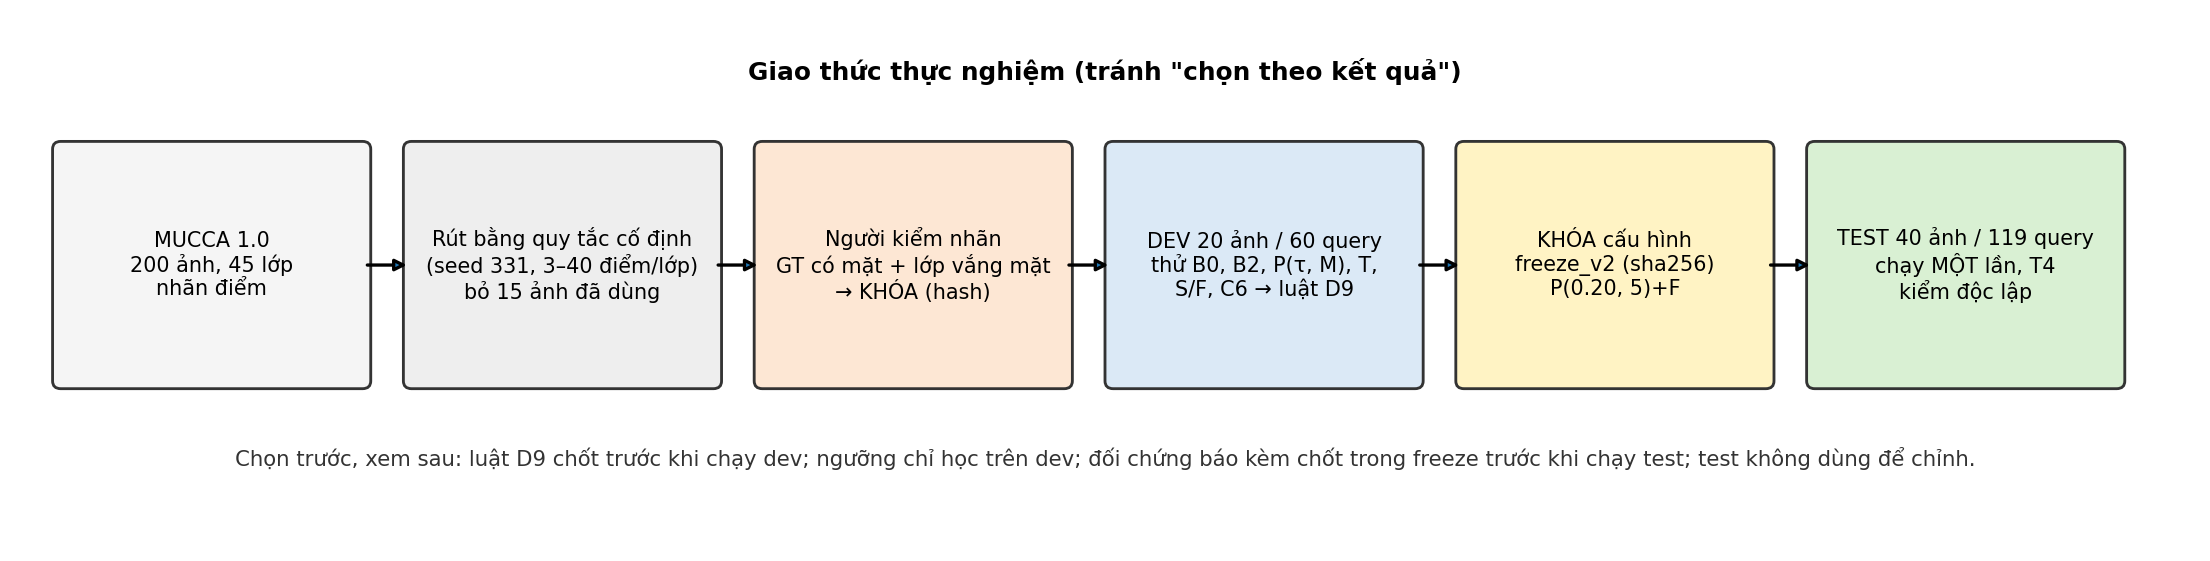
\includegraphics[width=\textwidth]{fig_protocol.png}
\caption{Giao thức thực nghiệm: dữ liệu được kiểm và khóa, luật chọn chốt trước, chọn và khóa cấu hình trên dev, test chạy một lần.}
\label{fig:protocol}
\end{figure}

\begin{enumerate}
\item \textbf{Luật chọn D9}, chốt trước khi chạy dev: chọn cấu hình có MAE cả tập nhỏ nhất trên dev, với điều kiện MAE câu có mặt không lớn hơn của \Bzero{} và $\FPRabs$ không lớn hơn của \Bzero. Luật này ngăn việc ``đổi'' cải thiện ở câu vắng mặt bằng cách làm hỏng câu có mặt. Nếu không cấu hình nào đạt, nhóm báo kết quả âm.
\item Trên dev thử lưới $\tau\in\{0.18,\dots,0.28\}$, $M\in\{5,10\}$, cùng T, S, F và \Csix. Ngưỡng S và F được chọn lại riêng cho từng nguồn ngay trên dev.
\item Khóa cấu hình vào \path{freeze_v2_20261111.json} (kể cả min/max và ngưỡng), cùng 4 đối chứng báo kèm khai báo trước: \Bzero, \Btwo, \Csix, \BtwoF.
\item Chạy test một lần trên Kaggle T4 (Triệu chạy). Chấm bằng một script duy nhất đọc file khóa; kết quả được tính lại độc lập từ đầu ra thô bằng một script viết riêng và khớp tuyệt đối.
\item Kết quả xấu cũng không chạy lại. Đối chứng báo kèm được thảo luận nhưng không được đổi thành phương pháp chính sau khi xem test.
\end{enumerate}
Với ít dữ liệu và nhiều tham số ($\tau$, $M$, các ngưỡng), rất dễ vô tình chọn cấu hình khớp với ngẫu nhiên của tập đang nhìn. Khóa trước là cách giữ cho con số test là một ước lượng không bị thiên lệch bởi việc chọn.

\subsection{Kiểm tái lập}
Kiểm A: lượt 1 trong lần chạy P trùng với \Bzero{} chạy riêng. Kiểm C: \Btwo{} chạy lại trùng với \Btwo{} đã lưu (60/60 câu trên dev). Mọi so sánh chỉ giữa các cách trong cùng một lần chạy trên T4.

% ================================================================== 7
\section{Kết quả}\label{sec:results}

\subsection{Kiểm môi trường trên FSCD-147}
Chạy lại checkpoint \cgdpp{} trên 1.190 ảnh test FSCD-147 cho MAE 8.34 và RMSE 24.64; bài báo gốc báo 8.39 và 27.03 \parencite{aminiNaieni2025countgdpp}. Môi trường chạy được coi là đúng. Đây không phải cải tiến của nhóm.

\subsection{Pilot}
Trên 5 ảnh pilot (15 câu có mặt), \Bzero{} có MAE 19.4 và \Btwo{} có MAE 22.0; cả hai chỉ đúng tuyệt đối 1/15 câu. Xem bằng mắt cả 15 câu cho thấy \cgdpp{} đếm lẫn loại (ví dụ hỏi blackberries có 21 quả, \Btwo{} đếm 79) và chỉ 23/42 mẫu giả đúng loại. Kết luận \Btwo{} kém \Bzero{} ở pilot phụ thuộc mạnh vào một câu, nên pilot chỉ được dùng để đặt giả thuyết.

\subsection{Cải tiến v1 trên 10 ảnh mới}
Bản v1 lọc khung của \Btwo{} bằng điểm \cgdpp{} (ngưỡng 0.907) hoặc bằng điểm kết hợp 50/50; ngưỡng chọn trên pilot rồi khóa. \Cref{tab:v1} cho thấy bộ lọc kết hợp giảm mạnh báo nhầm vật vắng mặt nhưng bỏ khoảng một nửa vật đúng, nên ở câu có mặt \Bzero{} vẫn tốt nhất. Quan sát này dẫn tới thiết kế v2: sửa \emph{nguồn} lỗi (mẫu giả) thay vì chỉ lọc ở cuối.

\begin{table}[ht]
\centering
\caption{Cải tiến v1 trên p4\_unseen\_v1 (10 ảnh, 30 câu).}
\label{tab:v1}
\small
\begin{tabular}{@{}lrrrr@{}}
\toprule
Cách & MAE (30) $\downarrow$ & MAE có mặt (20) $\downarrow$ & Đếm TB câu vắng mặt $\downarrow$ & Khung sai loại $\downarrow$\\
\midrule
\Bzero & 6.77 & \textbf{5.70} & 8.9 & 106\\
\Btwo & 13.00 & 12.95 & 13.1 & 238\\
\Btwo{} + lọc điểm & 7.27 & 8.75 & 4.3 & 92\\
\Btwo{} + kết hợp & \textbf{5.53} & 7.80 & \textbf{1.0} & \textbf{31}\\
\bottomrule
\end{tabular}
\end{table}

\subsection{Review khung bằng người (N4)}
Triệu gán nhãn mù 117 khung của 7 câu lỗi được chọn có chủ đích; đây là phân tích lỗi, không phải mẫu đại diện. Ở các câu được hai người cùng xem, Trí và Triệu đồng ý 9/9. Các phát hiện chính: khung bộ lọc v1 giữ lại không có khung nào đúng loại (lọc điểm 0/78, kết hợp 0/14; ví dụ hỏi ``people'' thì 9/9 khung là chó); mẫu giả chỉ đúng loại 1/21 lần; ở ảnh mcac\_88, câu ``people'' và câu ``cars'' trả về 21/21 khung trùng nhau (IoU $\ge 0.8$); vật đúng có trong ứng viên nhưng bị lọc mất (13/18 ứng viên là người thật). Kết luận của N4 là lỗi bắt đầu từ mẫu giả và cách chấm lượt 2; từ đó nhóm chọn nhánh P làm hướng chính và giữ \Csix{} làm đối chứng bắt buộc.

\subsection{Dev v2}
\Cref{tab:dev} tóm tắt kết quả dev. Theo luật D9, cấu hình được chọn là P($\tau=0.20$, $M=5$)\,+\,F. Các cách đứng đầu rất sát nhau và ngưỡng được chọn ngay trên dev, nên con số dev là lạc quan.

\begin{table}[ht]
\centering
\caption{Kết quả trên dev v2 (20 ảnh, 60 câu).}
\label{tab:dev}
\small
\begin{tabular}{@{}lrrr@{}}
\toprule
Cách & MAE $\downarrow$ & MAE có mặt $\downarrow$ & $\FPRabs$ $\downarrow$\\
\midrule
\Bzero & 6.28 & 8.25 & 0.20\\
\Btwo & 9.15 & 12.00 & 0.20\\
\textbf{P($\tau$ 0.20, $M$ 5)\,+\,F} & \textbf{3.53} & 5.05 & \textbf{0.05}\\
P($\tau$ 0.18--0.22, $M$ 10)\,+\,F & 3.62--3.63 & 5.03--5.22 & 0.05--0.20\\
\BtwoF & 3.73 & 5.15 & 0.20\\
P+T+F & 3.78 & -- & --\\
\Csix{} = \Bzero{} + F & 4.02 & 5.80 & 0.05\\
T / P+T (không lọc) & 8.55 / 8.25 & -- & --\\
\bottomrule
\end{tabular}
\end{table}

\subsection{Kết quả cuối trên test}\label{sec:test}
Tập test có 40 ảnh và 119 câu được chấm (79 có mặt, 40 vắng mặt). \Cref{tab:test} và \cref{fig:test} là kết quả của lần chạy duy nhất.

\begin{table}[ht]
\centering
\caption{Kết quả test (40 ảnh, 119 câu). $\Delta$ là chênh lệch MAE so với \Bzero; khoảng tin cậy 95\% bootstrap theo ảnh. Chỉ \PF{} là cấu hình chính; các dòng còn lại là đối chứng khai báo trước.}
\label{tab:test}
\small
\begin{tabular}{@{}lrrrl@{}}
\toprule
Cách & MAE $\downarrow$ & MAE có mặt $\downarrow$ & $\FPRabs$ $\downarrow$ & $\Delta$ so với \Bzero{} [CI 95\%]\\
\midrule
\Bzero & 7.71 & 8.32 & 0.250 & --\\
\Btwo & 9.61 & 10.24 & 0.250 & $+1.90$ [$+0.81$, $+3.03$]\\
\textbf{\PF{} (chính, đã khóa)} & \textbf{5.82} & \textbf{6.84} & \textbf{0.225} & $\mathbf{-1.88}$ [$-3.66$, $-0.44$]\\
\midrule
\BtwoF{} (báo kèm) & 5.70 & 6.81 & 0.250 & $-2.01$ [$-3.94$, $-0.40$]\\
\Csix{} = \Bzero+F (báo kèm) & 4.63 & 6.48 & 0.100 & $-3.08$ [$-6.62$, $-0.51$]\\
\bottomrule
\end{tabular}
\end{table}

\begin{figure}[ht]
\centering
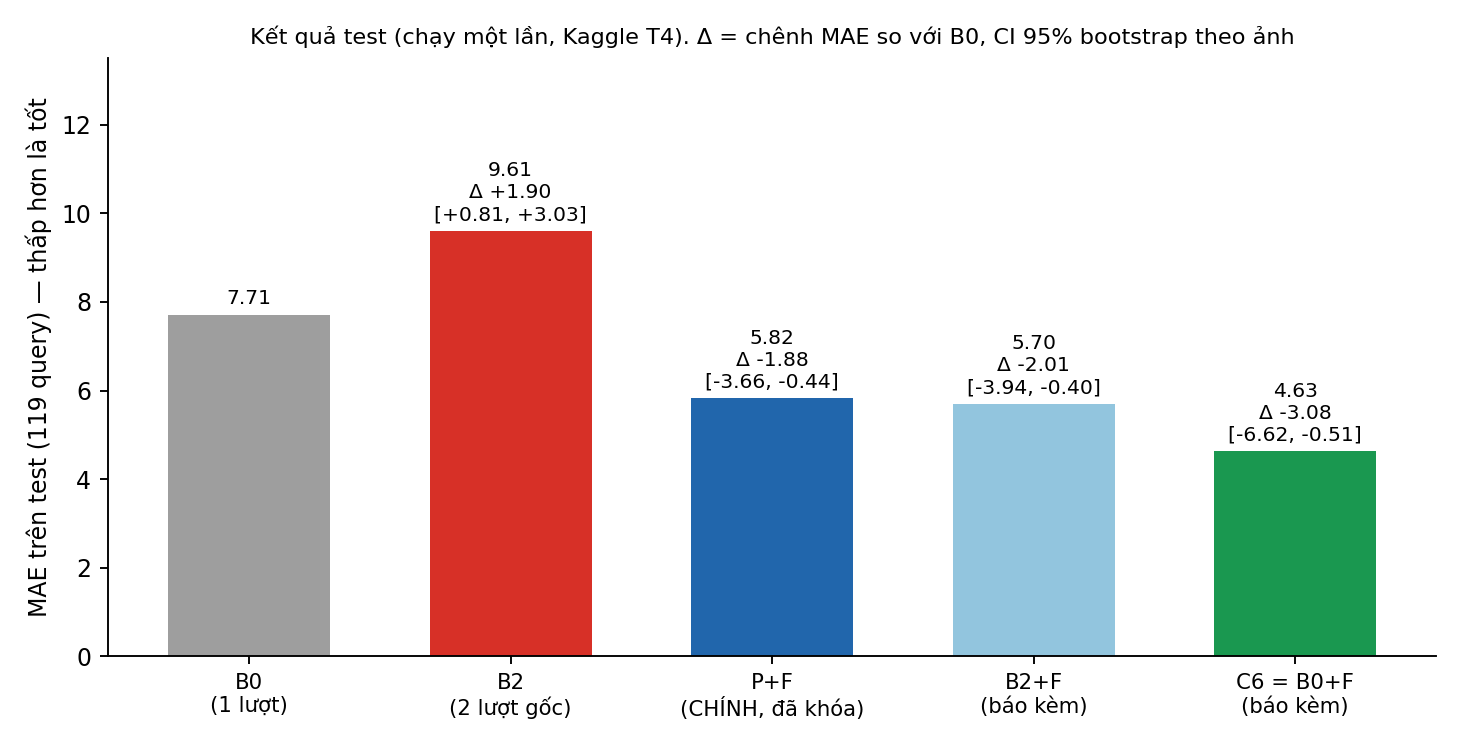
\includegraphics[width=0.78\textwidth]{fig_results_test.png}
\caption{MAE trên test của 5 cách được báo.}
\label{fig:test}
\end{figure}

So sánh cặp giữa các đối chứng: \Csix{} so với \PF{} là $-1.19$ [$-3.32$, $+0.24$], chưa đủ chắc; \BtwoF{} so với \PF{} là $-0.13$ [$-0.41$, $+0.18$], gần như bằng nhau. Bảng độ nhạy D11 (thay đáp án bằng số người kiểm đếm) làm MAE thay đổi dưới 0.06 và không đổi thứ tự.

\textbf{Trả lời RQ3.} So với \cgdpp{} một lượt (so sánh chính khai báo trước), cấu hình đã khóa giảm MAE 24\% (7.71 $\to$ 5.82), khoảng tin cậy 95\% không chứa 0. So với hai lượt gốc \Btwo, MAE giảm 39\% (9.61 $\to$ 5.82); phép so sánh cặp này không nằm trong kế hoạch kiểm định khai báo trước, nên chúng tôi chỉ báo như con số mô tả.

% ================================================================== 8
\section{Phân tích và thảo luận}\label{sec:analysis}

\subsection{Vì sao lượt 2 gây hại (RQ1)}
\Btwo{} kém \Bzero{} trên test với khoảng tin cậy không chứa 0; đây là lần thứ ba quan sát được điều này, sau pilot và p4\_unseen\_v1. Ở 79 câu có mặt, \Bzero{} đếm thừa tổng cộng 580 vật và thiếu 77; \Btwo{} đếm thừa 751 và thiếu 58. Lượt 2 làm số khung tăng thêm.

\Cref{tab:T} cho thấy bỏ cách chấm $\max$ (biến thể T) có giúp: trên dev, \Btwo{} $-$ \Tv{} $=+0.60$ [$+0.12$, $+1.23$]. Nhưng T vẫn kém \Bzero{} ở cả hai tập, và tỉ lệ tác hại T gỡ được dao động mạnh (21\% và 67\%). Chúng tôi chỉ kết luận được rằng cách chấm $\max$ giải thích \emph{một phần} tác hại của lượt 2; phần còn lại phù hợp với giả thuyết H2 nhưng H2 chưa được kiểm trực tiếp.

\begin{table}[ht]
\centering
\caption{Phép thử H1 bằng biến thể T (khoảng tin cậy tính sau test, bootstrap theo ảnh).}
\label{tab:T}
\small
\begin{tabular}{@{}lrrrll@{}}
\toprule
Tập & \Bzero & \Tv & \Btwo & Phần gỡ được $\frac{\Btwo-\Tv}{\Btwo-\Bzero}$ & \Tv{} so với \Bzero\\
\midrule
dev v2 (20 ảnh) & 6.28 & 8.55 & 9.15 & \textbf{21\%} [5\%, 60\%] & $+2.27$ [$+0.52$, $+4.12$]\\
p4\_unseen\_v1 (10 ảnh) & 6.77 & 8.80 & 13.00 & 67\% & $+2.03$ [$-0.37$, $+5.33$]\\
\bottomrule
\end{tabular}
\end{table}

\subsection{Vì sao P không đóng góp thêm \hk}
P chọn đúng y hệt bộ mẫu của \Btwo{} ở 108/120 câu (90\%). Cách giải thích hợp lý nhất: với $M=5$, khi 3 ứng viên điểm cao nhất đều qua ngưỡng CLIP $\tau=0.20$ (một ngưỡng khá thấp), P chọn lại đúng 3 khung đó. Theo cách kiểm điểm nhãn dễ dãi, tỉ lệ mẫu trúng đúng loại chỉ tăng từ 82\% (\Btwo) lên 85\% (P). P đúng hướng nhưng quá nhẹ tay để thay đổi đầu vào lượt 2, và không chạm tới cơ chế $\max$. Điều này giải thích vì sao \BtwoF{} $\approx$ \PF.

\subsection{Bộ lọc F thật sự làm gì \hk}
\begin{table}[ht]
\centering
\caption{Khung được giữ theo điểm nhãn (79 câu có mặt) và tỉ lệ khung dùng chung X/Y (IoU $\ge 0.5$, 39 ảnh, CI 95\%).}
\label{tab:boxes}
\small
\begin{tabular}{@{}lrrrrl@{}}
\toprule
Cách & Khung giữ & Đúng loại & Chỉ loại khác & Không trúng & Dùng chung X/Y\\
\midrule
\Bzero & 1481 & 60.4\% & 34.6\% & 5.1\% & 64\% [51, 75]\\
\Btwo & 1671 & 56.6\% & 34.6\% & 8.8\% & 71\% [58, 81]\\
\PF & 924 & 66.3\% & 32.7\% & 1.0\% & 59\% [40, 74]\\
\BtwoF & -- & -- & -- & -- & 59\% [41, 73]\\
\Csix & 746 & \textbf{76.9\%} & \textbf{21.3\%} & 1.7\% & \textbf{24\%} [11, 37]\\
\bottomrule
\end{tabular}
\end{table}

\Cref{tab:boxes} cho thấy: áp sau lượt 2, F chủ yếu dọn khung không chứa vật (8.8\% $\to$ 1.0\%) nhưng chưa tách được X với Y: vẫn khoảng 1/3 khung là vật loại khác và 59\% khung dùng chung. Áp ngay sau lượt 1 (\Csix), F tách rõ hơn (24\% dùng chung, 21\% sai loại). Về hướng của lỗi, sau F tổng đếm thừa giảm mạnh (\Bzero{} $+580$ $\to$ \PF{} $+243$) nhưng đếm thiếu tăng ($-77$ $\to$ $-297$): F đổi lỗi đếm thừa thành đếm thiếu, vì nó bỏ các khung ``không chắc'' và trong đó có cả vật đúng. Với câu vắng mặt, 92--100\% khung đếm nhầm nằm trên một vật khác có thật trong ảnh, không phải trên nền: mô hình ``trỏ lại'' vào vật có sẵn thay vì trả 0.

\subsection{Kết quả theo loại cặp \hk}
\begin{figure}[ht]
\centering
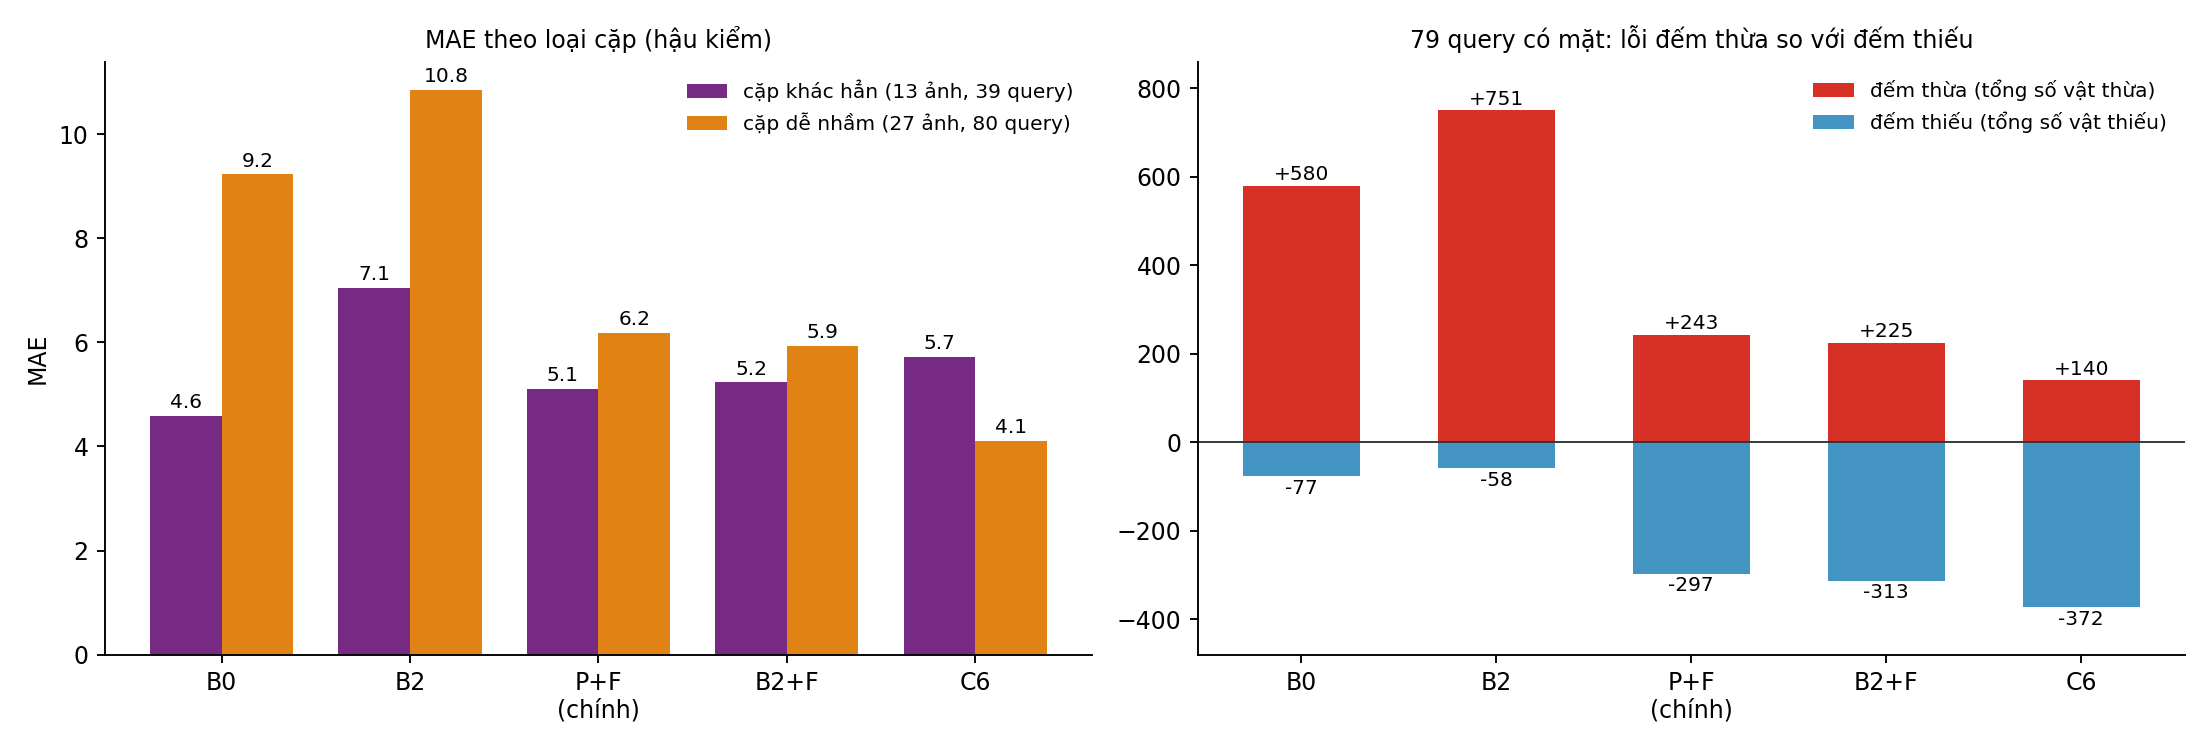
\includegraphics[width=\textwidth]{fig_strata_errors.png}
\caption{MAE theo loại cặp và phân rã đếm thừa/đếm thiếu trên test.}
\label{fig:strata}
\end{figure}

\begin{table}[ht]
\centering
\caption{MAE theo loại cặp trên test; $\Delta$ so với \Bzero{} [CI 95\%].}
\label{tab:strata}
\small
\begin{tabular}{@{}lll@{}}
\toprule
Cách & Cặp khác hẳn (13 ảnh) & Cặp dễ nhầm (27 ảnh)\\
\midrule
\Bzero & 4.59 / -- & 9.23 / --\\
\Btwo & 7.05 / $+2.46$ [$+0.38$, $+4.74$] & 10.85 / $+1.63$ [$+0.39$, $+2.86$]\\
\PF & 5.10 / $+0.51$ [$-0.72$, $+1.82$] & \textbf{6.18 / $-3.05$} [$-5.43$, $-0.96$]\\
\BtwoF & 5.23 / $+0.64$ [$-0.85$, $+2.03$] & 5.93 / $-3.30$ [$-5.90$, $-1.05$]\\
\Csix & 5.72 / $+1.13$ [$-0.87$, $+3.51$] & \textbf{4.10 / $-5.13$} [$-10.16$, $-1.60$]\\
\bottomrule
\end{tabular}
\end{table}

Cải thiện đến từ cặp dễ nhầm (quả với quả, đĩa với bát), nơi \Bzero{} đếm thừa nhiều và bộ lọc có tác dụng rõ (\cref{tab:strata,fig:strata}). Với cặp khác hẳn như người--xe, đúng dạng câu hỏi X/Y ban đầu, \Bzero{} đã khá tốt (MAE 4.59), các cách lọc chưa cho khác biệt chắc chắn và có xu hướng đếm thiếu ở câu có mặt (MAE có mặt: \Bzero{} 3.54, \PF{} 6.12, \Csix{} 8.50); đổi lại, \Csix{} giảm báo nhầm vật vắng mặt ở nhóm này ($\FPRabs$ 0.46 $\to$ 0.08). Nhóm cặp khác hẳn chỉ có 13 ảnh, nên mọi nhận xét ở đây thiếu lực thống kê.

\subsection{Ví dụ minh họa}
Trong các hình dưới, khung xanh trúng đúng loại, khung đỏ chỉ trúng loại khác, khung xám không chứa điểm nhãn nào; chấm trắng là điểm nhãn của loại được hỏi.

\begin{figure}[H]
\centering
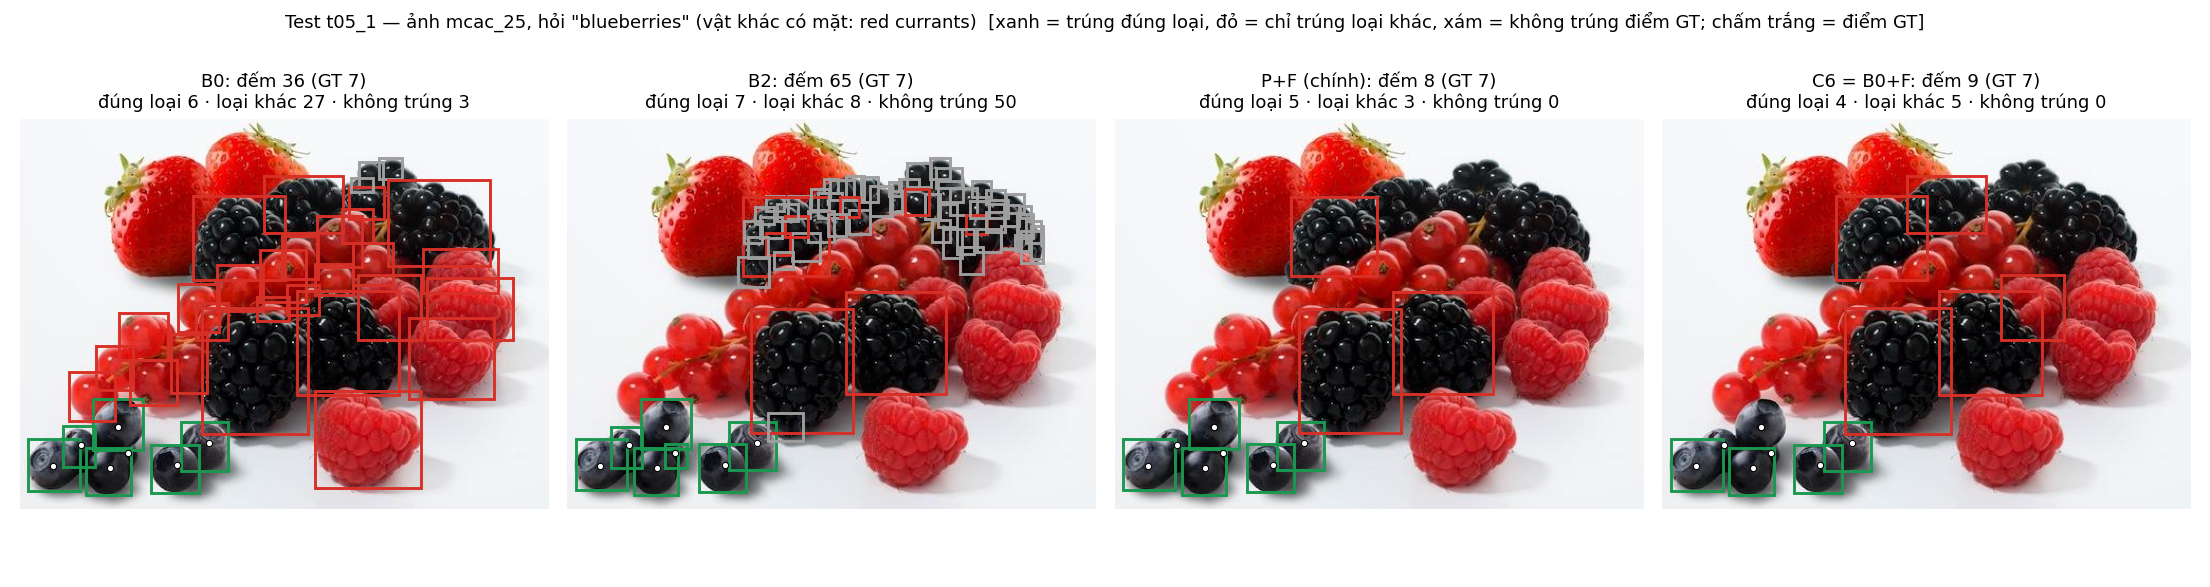
\includegraphics[width=\textwidth]{fig_example_t05_1_mcac_25.png}
\caption{Thành công: ``blueberries'' (đáp án 7). \Bzero{} 36, \Btwo{} 65, \PF{} 8, \Csix{} 9. \Btwo{} thêm khoảng 50 khung xám là từng hạt của quả mâm xôi đen.}
\label{fig:ex-success}
\end{figure}
\begin{figure}[H]
\centering
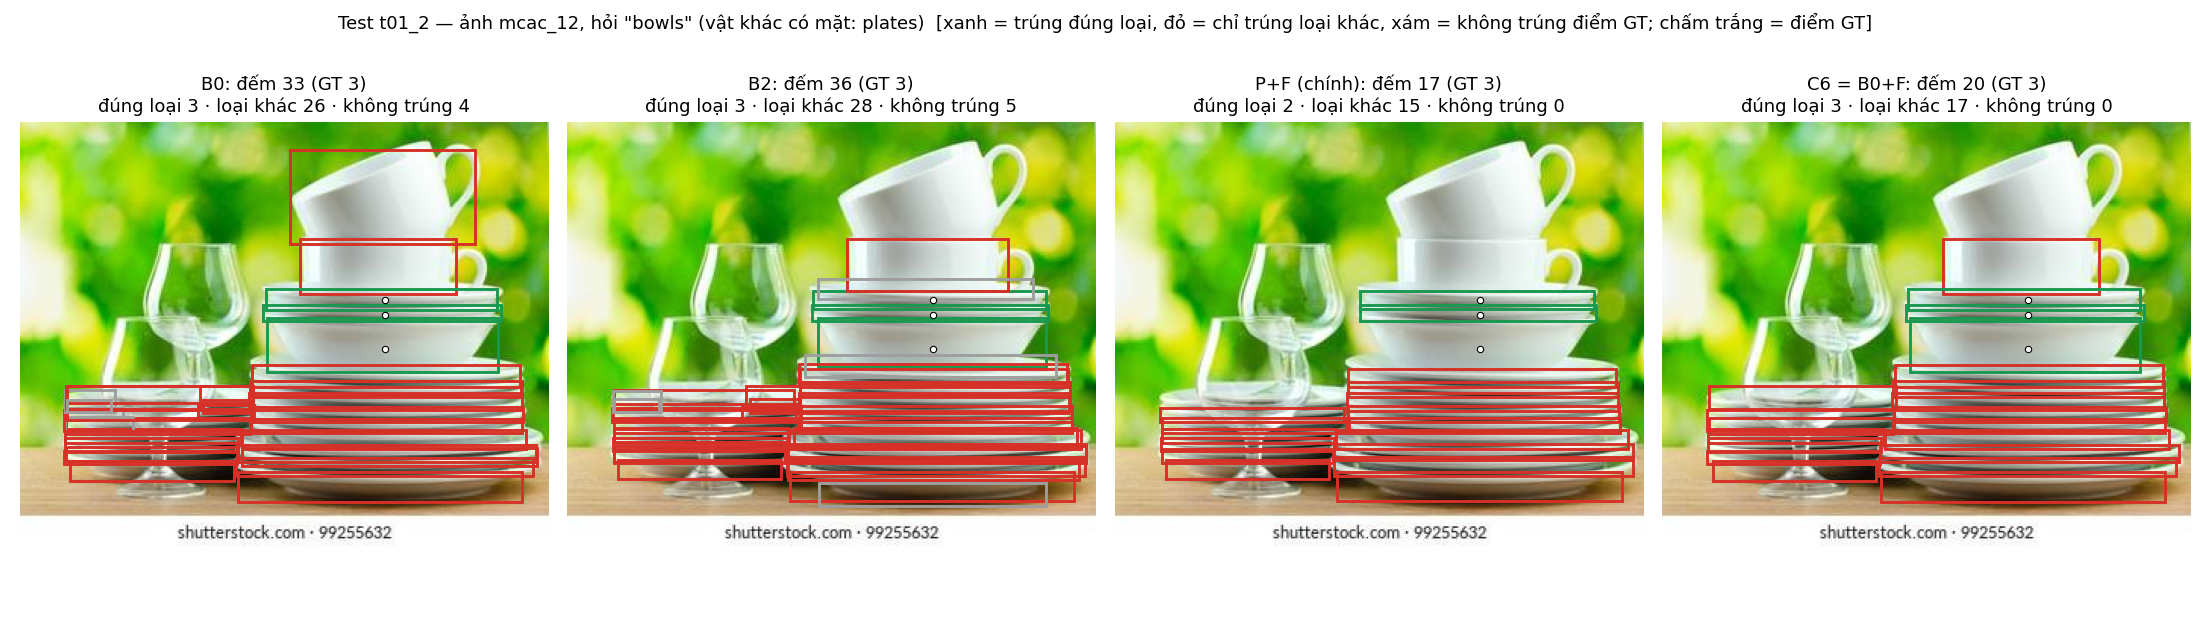
\includegraphics[width=\textwidth]{fig_example_t01_2_mcac_12.png}
\caption{Lỗi X/Y còn lại: ``bowls'' (đáp án 3). Chồng đĩa bị đếm là bát ở mọi cách (\PF{} 17, \Csix{} 20).}
\label{fig:ex-bowls}
\end{figure}
\begin{figure}[H]
\centering
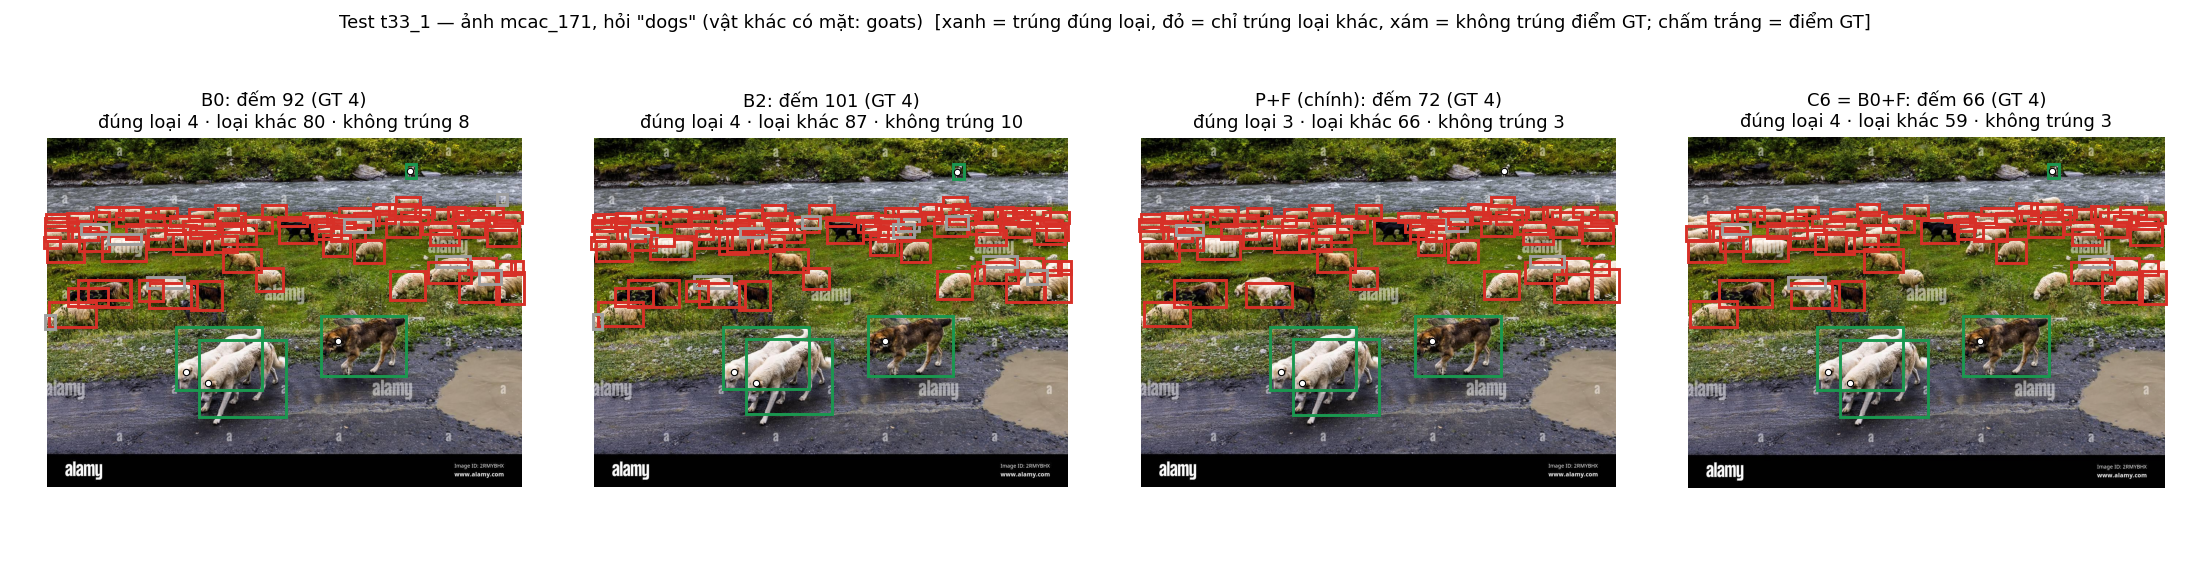
\includegraphics[width=\textwidth]{fig_example_t33_1_mcac_171.png}
\caption{Thất bại: ``dogs'' (đáp án 4). Đàn dê bị đếm là chó (66--101) ở mọi cách; CLIP không tách được dê với chó ở các ô ảnh nhỏ.}
\label{fig:ex-dogs}
\end{figure}
\begin{figure}[H]
\centering
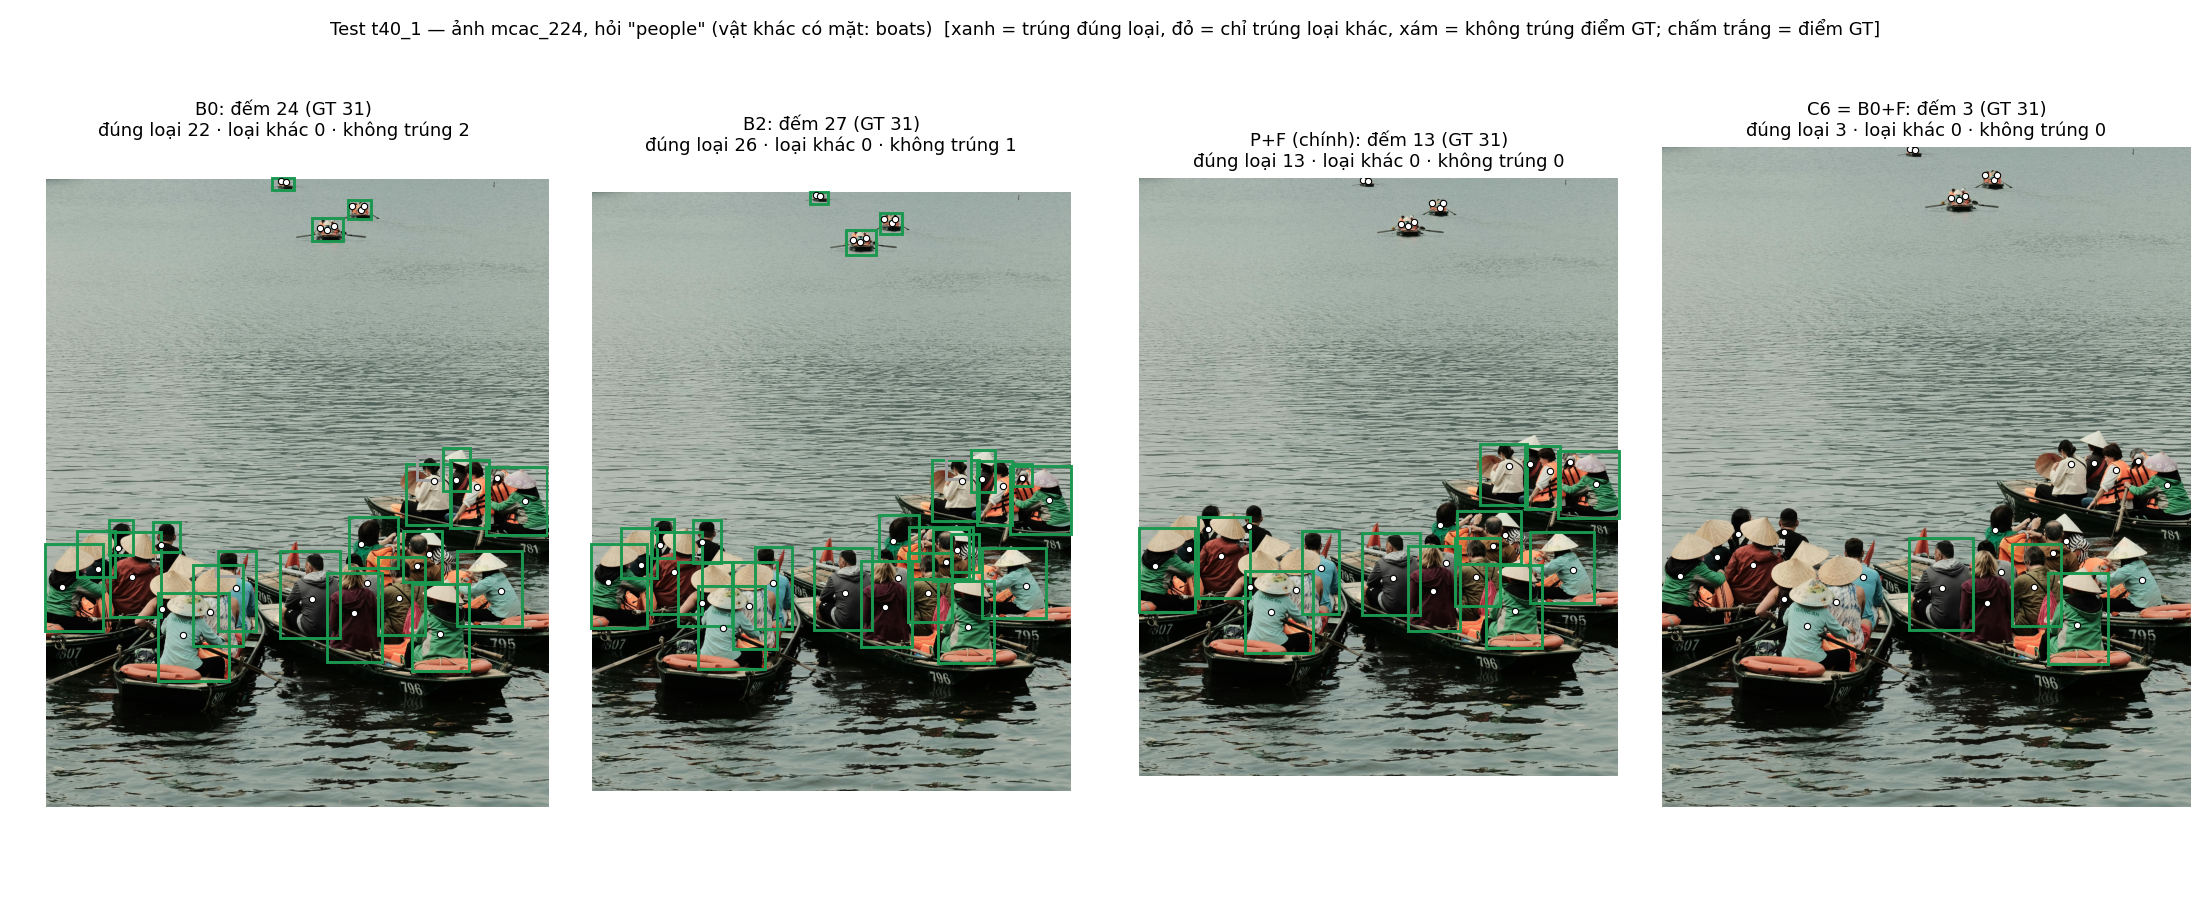
\includegraphics[width=\textwidth]{fig_example_t40_1_mcac_224.png}
\caption{Lọc quá tay: ``people'' (đáp án 31). Không có khung sai loại, nhưng F bỏ cả người thật (\PF{} 13, \Csix{} 3).}
\label{fig:ex-people}
\end{figure}

\subsection{Thứ hạng của \Csix{} và bài học về chọn cấu hình}\label{sec:c6}
Trên dev, \Csix{} chỉ đứng thứ 25/90 cấu hình riêng lẻ (thứ 7/15 khi gom theo họ phương pháp), nhưng trên test nó có MAE thấp nhất trong 5 cách được báo. Thứ hạng test chỉ tính 5 cách khai báo trong file khóa, nên không so trực tiếp được với thứ hạng dev. Chúng tôi xếp các giải thích từ chắc nhất tới ít chắc nhất:
\begin{enumerate}
\item \textbf{Thứ hạng nằm trong nhiễu.} \Csix{} $-$ \PF{} có khoảng tin cậy chứa 0 ở cả dev ($+0.48$ [$-0.62$, $+1.63$]) và test ($-1.19$ [$-3.32$, $+0.24$]). Bảy họ đứng đầu trên dev chỉ cách nhau 0.49 MAE, trong khi một khoảng tin cậy điển hình rộng khoảng 2.
\item \textbf{Lạc quan do chọn.} Luật D9 lấy cấu hình có MAE dev nhỏ nhất trong khoảng 80 cấu hình gần bằng nhau trên cùng 60 câu, nên cấu hình thắng thường là cấu hình ``gặp may'' nhất. Số liệu khớp với giải thích này (\cref{tab:devtest}): test khó hơn dev một chút (\Bzero{} tăng $+1.42$), nhưng cấu hình thắng dev hụt nhiều nhất ($+2.29$), còn \Csix{} hụt ít nhất ($+0.61$).
\item \textbf{Số lựa chọn khác nhau.} \Csix{} chỉ chọn 5 con số của bộ lọc F; \PF{} chọn thêm $\tau$, $M$ và đi qua lượt 2.
\item \textbf{Cơ chế.} \Csix{} lọc khung trước khi lượt 2 kịp thêm khung theo mẫu giả, nên tách X/Y tốt hơn (\cref{tab:boxes}).
\end{enumerate}

\begin{table}[ht]
\centering
\caption{MAE từ dev sang test.}
\label{tab:devtest}
\small
\begin{tabular}{@{}lrrr@{}}
\toprule
Cách & Dev & Test & Thay đổi\\
\midrule
\Bzero{} (không chọn tham số) & 6.28 & 7.71 & $+1.42$\\
\PF{} (thắng D9) & 3.53 & 5.82 & $+2.29$\\
\BtwoF & 3.73 & 5.70 & $+1.96$\\
\Csix & 4.02 & 4.63 & $+0.61$\\
\bottomrule
\end{tabular}
\end{table}

Bài học: khi các cách đứng đầu trên dev nằm trong cùng khoảng nhiễu, nên ưu tiên cách đơn giản hơn (tương tự ``quy tắc một sai số chuẩn''), hoặc dùng dev lớn hơn hay kiểm chéo. Nhóm không đổi kết quả chính sau khi xem test; \Csix{} được ghi nhận như một giả thuyết cho lần kiểm sau trên dữ liệu mới, kèm lưu ý ở \cref{sec:fsc147} rằng \Csix{} kém nhất trên ảnh FSC-147 đông vật.

\subsection{Chi phí tính toán}
Trên Kaggle T4, \Bzero{} mất khoảng 0.89 giây/câu; \Btwo{} và P khoảng 1.5 giây/câu (lượt 2 chạy ở khoảng 70\% số câu), chưa tính CLIP. \Csix{} bỏ được lượt 2 nên tiết kiệm khoảng 40\% thời gian \cgdpp. Thời gian CLIP chỉ được đo ở khảo sát FSC-147: khoảng 1.3 giây/câu (404.1 giây cho 300 câu), trên ảnh trung bình 66 vật nên nhiều khung hơn ảnh MUCCA; đây chỉ là mức tham khảo.

\subsection{Khảo sát bổ sung trên 300 ảnh FSC-147}\label{sec:fsc147}
\textbf{Mục đích.} Kiểm xem trên ảnh \emph{một loại vật}, giữ hay bỏ lượt 2 tốt hơn, và cấu hình đã khóa đứng ở đâu. Thiết kế được khai báo trước (\path{experiments/fsc147_survey/KHAI_BAO_TRUOC_FSC147_20261120.md}): mẫu cố định 300 ảnh FSC-147 test (seed 331), mọi câu đều có mặt; một lần chạy trên Kaggle T4, không cắt ảnh, không dùng mẫu sinh bởi mô hình ngôn ngữ; tham số giữ nguyên từ file khóa v2; so sánh chính là \Bzero{} $-$ \Btwo{} với bootstrap ghép cặp theo ảnh. Kiểm A của notebook đạt (lệch lớn nhất $3.28\times10^{-7}$), và toàn bộ số đếm, chỉ số, khoảng tin cậy được tính lại bằng một script độc lập, không dùng code chấm của repo, và đều khớp.

\begin{table}[ht]
\centering
\caption{Khảo sát 300 ảnh FSC-147 (chỉ câu có mặt).}
\label{tab:fsc}
\small
\begin{tabular}{@{}lrrrrr@{}}
\toprule
Cách & MAE $\downarrow$ & Bias & Thừa / thiếu & MAE ($\le$40 vật) & MAE ($>$40 vật)\\
\midrule
\Bzero & 13.88 & $-1.54$ & 1851 / 2312 & 3.95 & 25.69\\
\Btwo & \textbf{13.32} & $-0.23$ & 1964 / 2033 & \textbf{3.44} & \textbf{25.09}\\
\PF{} (đã khóa) & 18.01 & $-14.68$ & 500 / 4904 & 3.50 & 35.28\\
\BtwoF & 17.98 & $-14.79$ & 478 / 4915 & 3.65 & 35.02\\
\Csix & 25.11 & $-20.93$ & 627 / 6907 & 5.34 & 48.64\\
\bottomrule
\end{tabular}
\end{table}

Các so sánh khai báo trước cho: \Bzero{} $-$ \Btwo{} (so sánh chính) $+0.55$ [$-3.00$, $+4.30$]; \PF{} $-$ \Btwo{} $+4.69$ [$+2.25$, $+7.50$]; \PF{} $-$ \Bzero{} $+4.14$ [$+0.56$, $+8.09$]. Như vậy trên ảnh một loại, giữ hay bỏ lượt 2 chưa khác nhau rõ, nên kết luận ``lượt 2 gây hại'' chỉ áp dụng cho ảnh nhiều loại. Cấu hình đã khóa kém hơn, chủ yếu ở ảnh trên 40 vật, vì bộ lọc F (chọn trên ảnh MUCCA 3--40 vật) bỏ cả vật đúng: \PF{} đếm thiếu 4904 vật so với 2033 của \Btwo; ở ảnh tối đa 40 vật, \PF{} ngang \Btwo. Phạm vi áp dụng của cải tiến vì vậy là ảnh nhiều loại, ít đến vừa vật. Khảo sát chỉ đúng cho mẫu và điều kiện này, không phải benchmark đầy đủ, không nói gì về lớp vắng mặt, và không so được với các số 8.34 / 8.39 vốn chạy với cắt ảnh và mẫu bổ sung trên đủ 1.190 ảnh.

\subsection{Thử nghiệm sơ bộ: gán khung theo CLIP giữa các loại (chỉ dev)}\label{sec:xyclip}
\textbf{Mục đích.} Thử một hướng nhắm thẳng vào việc hỏi X mà trả về khung của Y. \textbf{Cách làm (bước A, không có tham số):} với mỗi khung đang được giữ, CLIP so ô cắt với tên các loại được hỏi trên cùng ảnh (X, Y, Z); khung chỉ được giữ nếu giống loại được hỏi nhất. Thử nghiệm được khai báo trước (\path{experiments/xy_clip_assign/KHAI_BAO_TRUOC_XY_CLIP_20261122.md}), chỉ chạy trên dev 20 ảnh, không chạy trên test; điểm CLIP tính lại trên CPU khớp điểm đã tính trên Kaggle (lệch lớn nhất $1.37\times10^{-6}$).

\begin{table}[ht]
\centering
\caption{Gán khung theo CLIP trên dev (20 ảnh).}
\label{tab:xyclip}
\small
\begin{tabular}{@{}lrr@{}}
\toprule
Chỉ số & \PF{} (đã khóa) & \PF{} + bước A\\
\midrule
Khung dùng chung X/Y $\downarrow$ & 61.6\% & \textbf{2.9\%}\\
Khung đúng loại $\uparrow$ & 70.2\% & 83.0\%\\
$\FPRabs$ $\downarrow$ & 0.05 & 0.00\\
MAE câu có mặt $\downarrow$ & \textbf{5.05} & 6.92\\
Đếm thừa / thiếu (câu có mặt) & 76 / 126 & 19 / 258\\
\bottomrule
\end{tabular}
\end{table}

So sánh chính khai báo trước cho khung dùng chung $-0.587$ [$-0.735$, $-0.404$] và MAE câu có mặt $+1.88$ [$-0.03$, $+3.73$]: đọc theo khai báo là một \emph{đánh đổi}. Bước A tách X/Y gần như hoàn toàn và có chọn lọc (bỏ 67\% khung sai loại, 127 $\to$ 42, nhưng chỉ 30\% khung đúng loại, 327 $\to$ 230). Tuy vậy 30\% vật đúng bị bỏ nhầm làm đếm thiếu tăng gấp đôi, nên số đếm không tốt hơn. Chỗ nghẽn vì vậy nằm ở độ tin cậy của CLIP trên ô cắt nhỏ với các loại gần nghĩa, không nằm ở luật gán. Đây chỉ là kết quả sơ bộ: dev đã được dùng để chọn F, và bước A giả định biết các loại khác được hỏi trên cùng ảnh.

% ================================================================== 9
\section{Hạn chế}\label{sec:limits}
\begin{enumerate}
\item \textbf{Cỡ mẫu nhỏ:} 40 ảnh test, trong đó chỉ 13 ảnh cặp khác hẳn; khoảng tin cậy rộng; các nhận xét theo loại cặp là hậu kiểm và chỉ mang tính mô tả.
\item \textbf{Một nguồn dữ liệu cho kết quả chính} (MUCCA). Khảo sát FSC-147 chỉ có câu có mặt và không cắt ảnh, nên chưa phải kiểm chứng đầy đủ trên nguồn khác.
\item \textbf{Nhãn:} đáp án là số điểm MUCCA; 15/120 câu test có ghi chú cần xem lại (bảng độ nhạy không đổi kết luận). Phép kiểm ``điểm trong khung'' là xấp xỉ dễ dãi; review N4 cho thấy phép kiểm tự động lạc quan hơn người kiểm.
\item \textbf{Ngưỡng cố định toàn cục:} F dùng một ngưỡng cho mọi ảnh, nên ảnh đông vật bị lọc quá tay (\cref{sec:fsc147}).
\item \textbf{Giới hạn của CLIP:} với ô cắt nhỏ và loại gần nghĩa (dê--chó--cừu, chồng đĩa--bát), điểm CLIP không đủ để tách loại (\cref{fig:ex-dogs,sec:xyclip}).
\item \textbf{Lạc quan do chọn trên dev:} thứ hạng dev không giữ được trên test (\cref{sec:c6}).
\item \textbf{Cơ chế lượt 2 chưa giải thích hết:} phân tích T dựa trên dev và tập chẩn đoán, chưa có T trên test; H2 chưa kiểm.
\item \textbf{Bài toán X/Y chưa giải xong:} sau cải tiến, MAE câu có mặt (6.84) vẫn khoảng một nửa số vật thật trung bình (12.4 vật), và \PF{} vẫn dùng chung 59\% khung giữa X và Y.
\end{enumerate}

% ================================================================== 10
\section{Kết luận và hướng phát triển}\label{sec:conclusion}
\textbf{RQ1.} Trong ảnh nhiều loại, \cgdpp{} thường trả về cùng một nhóm khung dù đổi câu hỏi (64\% khung dùng chung giữa X và Y), và khoảng 1/3 khung là vật loại khác. Cơ chế hai lượt tự chọn mẫu làm lỗi nặng thêm; cách chấm $\max$ ở lượt 2 chỉ giải thích một phần (khoảng 1/5 trên dev).

\textbf{RQ2.} Có thể giảm lỗi mà không huấn luyện lại. Thành phần hiệu quả là lọc khung bằng điểm kết hợp \cgdpp{} + CLIP; kiểm mẫu bằng CLIP (P) với ngưỡng đã chọn gần như không đổi bộ mẫu.

\textbf{RQ3.} Trên test khóa trước, cấu hình chính giảm MAE 24\% so với một lượt, với khoảng tin cậy 95\% không chứa 0. Cải thiện tập trung ở cặp dễ nhầm và đi kèm xu hướng đếm thiếu.

\textbf{Phạm vi áp dụng.} Trên 300 ảnh FSC-147 một loại, cấu hình đã khóa kém hơn \cgdpp{} gốc, chủ yếu ở ảnh đông vật. Cải tiến dành cho ảnh nhiều loại, ít đến vừa vật; ngay cả trong phạm vi đó, bài toán X/Y mới được giảm nhẹ.

\textbf{Hướng phát triển} (đều cần một tập kiểm mới, độc lập):
\begin{enumerate}
\item Kiểm \Csix{} (lọc ngay sau lượt 1) kèm ngưỡng theo mật độ vật.
\item Chỉ dùng CLIP phân xử các khung bị câu X và câu Y tranh nhau, giữ nguyên các khung khác; dùng bộ kiểm mạnh hơn (CLIP lớn hơn, ô cắt có ngữ cảnh).
\item Ngưỡng thích ứng theo mật độ vật để tránh lọc quá tay ở ảnh đông.
\item Kiểm giả thuyết H2 bằng cách so điểm token chữ của cùng khung ở lượt 1 và lượt 2.
\item Dùng câu chỉ định ``không đếm Y'' có sẵn trong \cgdpp{} khi hỏi X.
\end{enumerate}

% ================================================================== Declarations
\section*{Đóng góp của thành viên}
\addcontentsline{toc}{section}{Đóng góp của thành viên}
\begin{table}[H]
\centering
\small
\begin{tabularx}{\textwidth}{@{}l L L@{}}
\toprule
Mảng & Đào Xuân Minh Trí & Triệu\\
\midrule
Môi trường & Dựng \cgdpp{} trên Kaggle T4, benchmark FSCD-147 & Kiểm chéo bộ chấm, tính tay, self-test\\
Pilot, v1 & Pilot 5 ảnh, xem bằng mắt 15 câu; cải tiến v1 & Tự kiểm kết quả v1\\
Chẩn đoán & Chẩn đoán điểm token; quyết định đưa biến thể T vào trước khi khóa & Review mù 117 khung (N4) và rà soát N4\\
Dữ liệu v2 & Kiểm 20 ảnh dev & Rút dev/test, kiểm 40 ảnh test, khóa dữ liệu\\
Thực nghiệm & Chọn và khóa cấu hình & Chạy dev, test một lần và khảo sát FSC-147 trên Kaggle\\
Viết & Bản chi tiết, bản tóm tắt gửi giảng viên & Công trình liên quan, so sánh với nhóm khác\\
\bottomrule
\end{tabularx}
\end{table}
\noindent\todo{Trí và Triệu cùng xác nhận bảng này trước khi nộp.}

\section*{Khai báo sử dụng công cụ AI}
\addcontentsline{toc}{section}{Khai báo sử dụng công cụ AI}
\todo{bản nháp, Trí và Triệu chốt câu chữ.} Nhóm sử dụng trợ lý AI (Claude) để hỗ trợ viết mã chấm điểm và phân tích hậu kiểm, tính lại độc lập các kết quả từ đầu ra thô, và soạn nháp tài liệu (bao gồm bản nháp báo cáo và slide này). Mọi quyết định thiết kế, kiểm nhãn bằng mắt, chạy mô hình trên Kaggle và lựa chọn cấu hình do nhóm thực hiện. Mọi con số trong báo cáo được đối chiếu với các tệp kết quả trong repo.

\printbibliography[heading=bibintoc,title={Tài liệu tham khảo}]

% ================================================================== Appendix
\appendix
\section{Nguồn số liệu trong repo}\label{app:sources}
\begin{table}[H]
\centering
\scriptsize
\begin{tabularx}{\textwidth}{@{}l X@{}}
\toprule
Mục & Tệp\\
\midrule
FSCD-147 & \path{reports/BENCHMARK_FSCD147.md}\\
Pilot & \path{reports/PILOT_SUMMARY.md}\\
v1 & \path{reports/P4_6_UNSEEN_RESULTS_20261027.md}\\
N4 & \path{reports/N4_KET_QUA_TANG_A_20261029.md}, \path{reports/RA_SOAT_TRIEU_N4_20261029.md}\\
Dev & \path{reports/DEV_V2_D9_KET_QUA_20261111.md}, \path{reports/TRIEU_W6_DEV_D9_20261111.md}\\
Test & \path{reports/KET_QUA_TEST_CUOI_20261111.md}, \path{results/countgdpp/p1_test_kaggle_t4_20261111_1430_eval/result.json}\\
T, thứ hạng \Csix & \path{results/countgdpp/p1_dev_kaggle_t4_20261111_1203_posthoc_20261115/summary.json}\\
Hậu kiểm test & \path{reports/PHAN_TICH_HAU_KIEM_TEST_20261111.md}, \path{results/countgdpp/p1_test_kaggle_t4_20261111_1430_posthoc_20261111/}\\
FSC-147 & \path{reports/TRIEU_FSC147_KHAO_SAT_20261122.md}, \path{results/countgdpp/fsc147_survey_kaggle_t4_20261122_1618*}\\
Gán khung CLIP & \path{reports/XY_CLIP_ASSIGN_DEV_KET_QUA_20261122.md}, \path{results/countgdpp/xy_clip_assign_dev_20261122_1755/}\\
Cấu hình khóa & \path{results/countgdpp/freeze_v2_20261111.json} (sha256 \texttt{64e89ef5\ldots})\\
Dữ liệu khóa & \path{experiments/countgdpp/dev_test_v2/}\\
Hình & \path{reports/figures/} (script \path{evaluation/make_report_figures.py})\\
\bottomrule
\end{tabularx}
\end{table}

\end{document}
